\section{NACA0012}
The last validation case from the TMR website is the NACA 0012 airfoil case, which was only run with NX Flow. This case is available on~\cite{tmr} under the name ``2D NACA 0012 airfoil''. While the Turbulence Modeling Resource provides grids for this problem, they are not suitable for the boundary conditions available in NX Flow. The mesh used is shown in~\Cref{fig:naca0012}, which is an unstructured mesh. The boundary layer is meshed with hexahedron elements and the far field with tetrahedral elements. The average value of $y^+$ for the first layer is approximately unity. No grid study was performed since no grid study data is available at~\cite{tmr}.
\begin{figure}
    \centering
    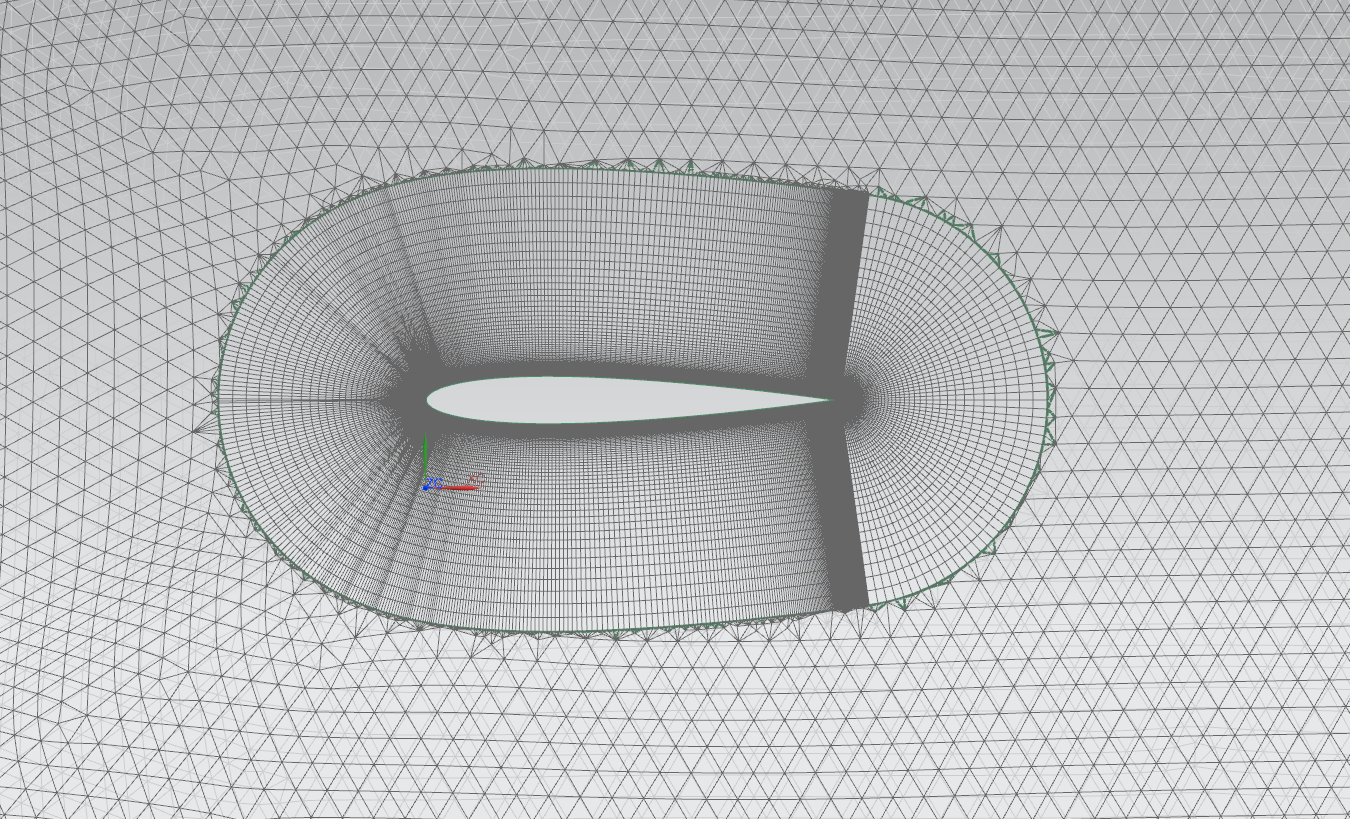
\includegraphics[width=0.5\textwidth]{figs/naca0012/naca0012.png}
    \caption{Close-up of the NACA0012 unstructured mesh. Far field extends 3 chords upstream, 7 chords downstream and 3 chords above and below.}
    \label{fig:naca0012}
\end{figure}
This case was run using a fixed density, as it is an incompressible case. The Reynolds number value is 6 million and three angles of attack were used: 0, 10 and 15 degrees.

\Cref{tab:naca0012} tabulates the lift and drag coefficients at all angles of attack and \Cref{fig:naca0012_0} through \Cref{fig:naca0012_15} compare the pressure and skin friction coefficient along the airfoil at $\alpha=0\degc$, $\alpha=10\degc$ and $\alpha=15\degc$ respectively. In all cases, there is a high level of suction on the upper surface at the leading edge, as the flow accelerates. The pressure differential between the upper and lower surface is, for the most part, what generates lift. The skin friction distribution is, as expected, qualitatively similar to that of the flat plate.

Even though there is decent agreement between the coefficients of pressure and skin friction, the drag values are heavily over-predicted by NX Flow. The pressure at the leading edge is under-predicted by NX Flow. Compounded with the fact that most of the drag (over 90\%) is due to the pressure forces in this case, this results in the large discrepancy observed.
\begin{table}
    \centering
    \caption{NACA0012: Comparison of drag and lift coefficients at all angles of attack.}
    \label{tab:naca0012}
    \begin{tabular}{@{}l cc c cc c cc@{}}
        \toprule
         & \multicolumn{2}{c}{$\alpha = 0\degc$} & \phantom{a}
            & \multicolumn{2}{c}{$\alpha = 10\degc$} & \phantom{a}
            & \multicolumn{2}{c}{$\alpha = 15\degc$}\\
        \cline{2-3} \cline{5-6} \cline{8-9}
        Code & $C_L$ & $C_D$ && $C_L$ & $C_D$ && $C_L$ & $C_D$ \\
        \midrule
        CFL3D & $\approx$ 0 & 0.00819 && 1.0909 & 0.01231 && 1.5461 & 0.02124 \\
        FUN3D & $\approx$ 0 & 0.00812 && 1.0983 & 0.01242 && 1.5547 & 0.02159 \\
        NX Flow & 7.5E-5    & 0.01230 && 1.0175 & 0.05018 && 1.4295 & 0.09959 \\
        \bottomrule
    \end{tabular}
\end{table}

\begin{figure}[ht!]
\centering
\begin{subfigure}{.45\textwidth}
  \centering
  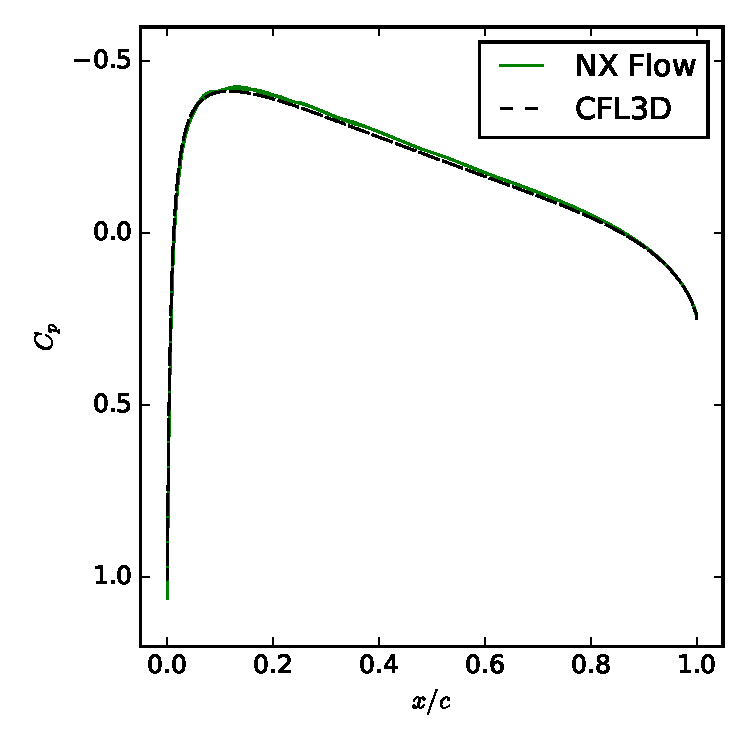
\includegraphics[width=1.0\textwidth]{figs/naca0012/cp_0.pdf}
  \caption{Coefficient of pressure.}
\end{subfigure}%
\begin{subfigure}{.45\textwidth}
  \centering
  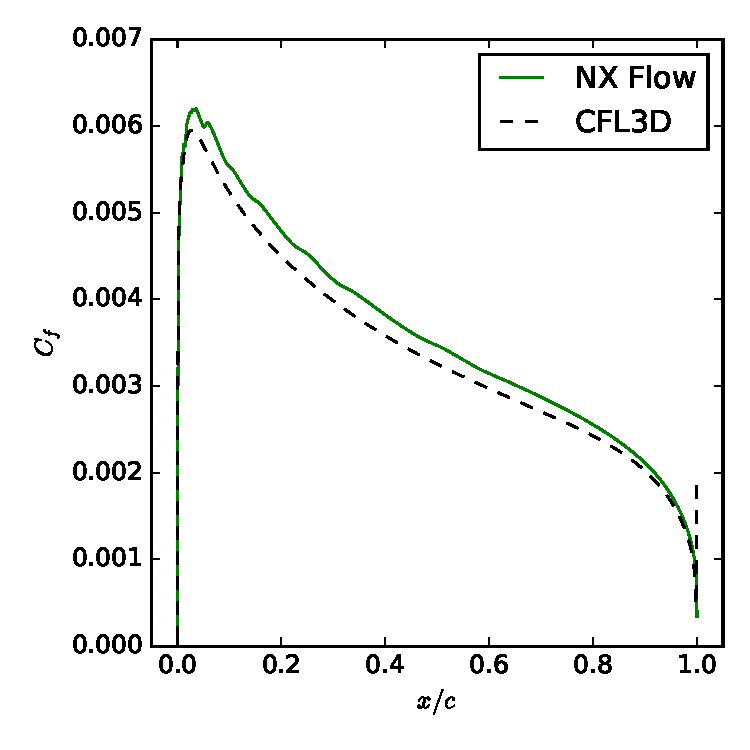
\includegraphics[width=1.0\textwidth]{figs/naca0012/cf_0.pdf}
  \caption{Coefficient of skin friction.}
\end{subfigure}
\caption{NACA0012 (NX Flow): Force coefficient distribution at $\alpha = 0\degc$.}
\label{fig:naca0012_0}
\end{figure}

\begin{figure}[ht!]
\centering
\begin{subfigure}{.45\textwidth}
  \centering
  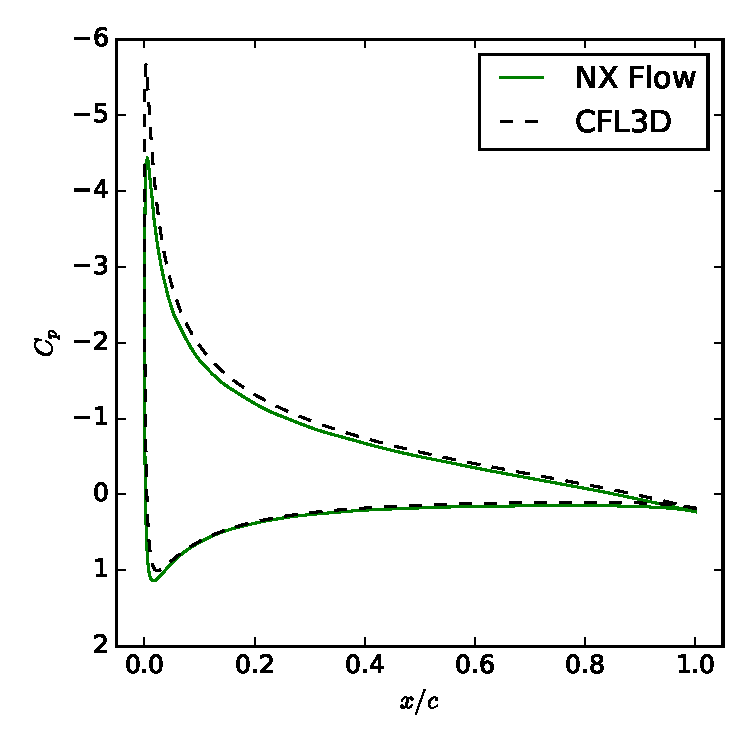
\includegraphics[width=1.0\textwidth]{figs/naca0012/cp_10.pdf}
  \caption{Coefficient of pressure.}
\end{subfigure}%
\begin{subfigure}{.45\textwidth}
  \centering
  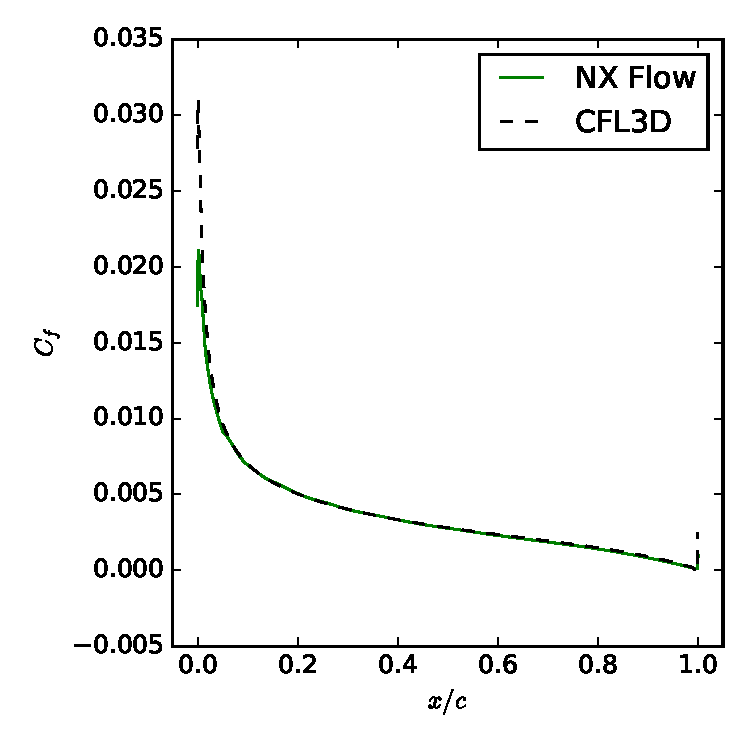
\includegraphics[width=1.0\textwidth]{figs/naca0012/cf_10.pdf}
  \caption{Coefficient of skin friction.}
\end{subfigure}
\caption{NACA0012 (NX Flow): Force coefficient distribution at $\alpha = 10\degc$.}
\label{fig:naca0012_10}
\end{figure}

\begin{figure}[ht!]
\centering
\begin{subfigure}{.45\textwidth}
  \centering
  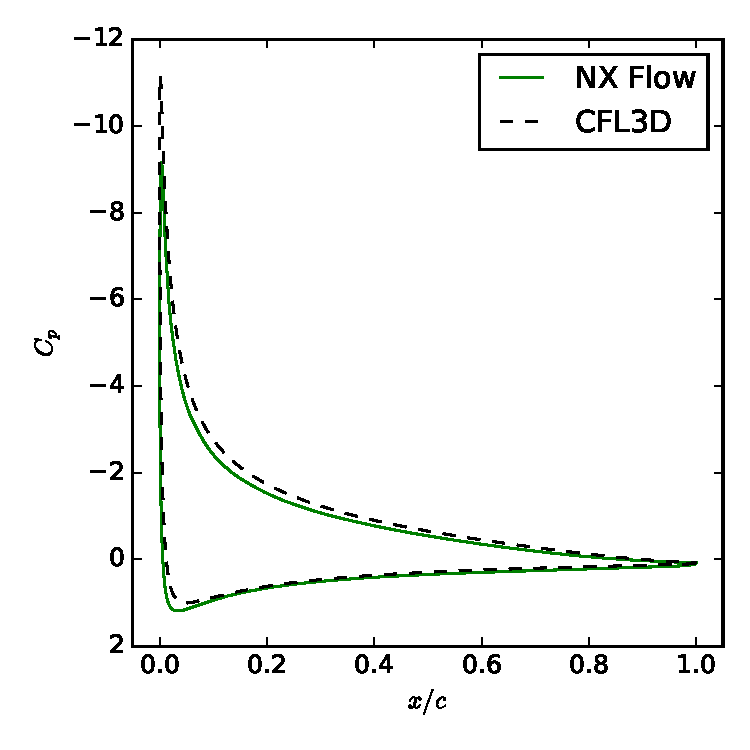
\includegraphics[width=1.0\textwidth]{figs/naca0012/cp_15.pdf}
  \caption{Coefficient of pressure.}
\end{subfigure}%
\begin{subfigure}{.45\textwidth}
  \centering
  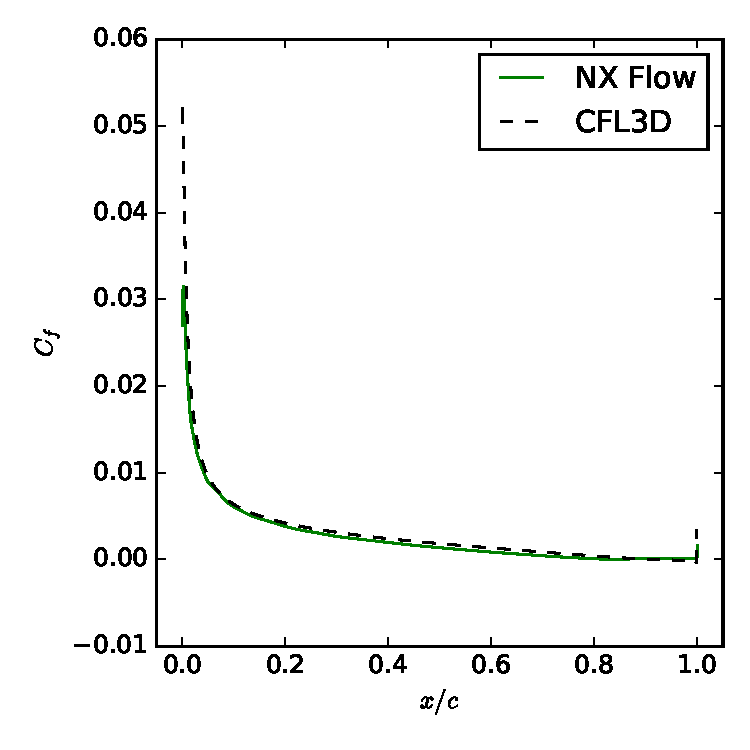
\includegraphics[width=1.0\textwidth]{figs/naca0012/cf_15.pdf}
  \caption{Coefficient of skin friction.}
\end{subfigure}
\caption{NACA0012 (NX Flow): Force coefficient distribution at $\alpha = 15\degc$.}
\label{fig:naca0012_15}
\end{figure}
